\phantomsection
\addcontentsline{toc}{chapter}{Introducción}
% Titulo de la introduccion.
\begin{center}
	{\bf Introducción} 
\label{chap:intro}
\end{center}

    Los humanos tienen la habilidad innata de relacionar los objetos que los
rodean con la información aprendida previamente. Esta habilidad les permite 
reconocer y clasificar de forma intuitiva di\-fe\-ren\-tes tipos de objetos. Sin
embargo, hacer que una computadora clasifique y reconozca objetos en grupos es
una tarea difícil.

    A medida que aumenta la cantidad de información con la que tienen que lidiar
los seres humanos, también crece la necesidad de poder procesarla y clasificarla
de manera automática. Por lo tanto, este problema ha sido ampliamente abordado
por investigadores en las área de estadística, inteligencia de negocios,
inteligencia artificial, etc\cite{SwAjAm2009}. Un componente fundamental
del área de inteligencia artificial es el reconocimiento de patrones donde uno de
sus objetivos es el de clasificar objetos en diferentes categorías o clases. Cuando
esta clasificación no es supervisada por un ser humano, se llama \emph{data
clustering}.

    El problema de \emph{Data clustering} es la clasificación no supervisada de
un conjunto de datos en grupos similares. Los datos pertenecientes a un grupo
(\emph{cluster}) tienen más similitudes entre sí, que con los datos pertenecientes
a otros grupos \cite{GaChJi2007}. Brucker en \cite{Br1978} demostró que el
problema es \emph{NP-hard} cuando el número de clusters excede a 3.

    Entre las aplicaciones de la resolución del problema de \emph{data clustering}
(minería de datos, segmentación de clientes, recuperación de documentos, etc.),
destaca el procesamiento de imágenes \cite{GaChJi2007}. Su importancia radica en
que el resultado de hacer \emph{data clustering} a una imagen puede ser usado
como entrada para una red neuronal de reconocimiento de objetos o de ayuda para
encontrar regiones de interés en imágenes médicas \cite{GaChJi2007}.

    Las metaheurísticas basadas en población e inteligencia colectiva
generalmente son apropiadas para resolver problemas \emph{NP-hard}, incluyendo
el problema de \emph{data clustering}, debido a que pueden evitar quedar atrapados
en soluciones óptimas locales y, normalmente, encuentran la solución óptima global
\cite{PSO_0}. Las metaheurísticas más conocidas y prometedoras son los algoritmos
genético \cite{DoGeGr2007}, de abeja\cite{BEE_0} y de hormiga\cite{Ant_0}\cite{OuBa2007},
el optimizador de enjambre de partículas \cite{PSO_0} y la evolución diferencial
\cite{SwAjAm2008}. Todas estas metaheurísticas funcionan con un grupo de individuos
que se mueven en un espacio de soluciones factibles del problema. La forma en
que se producen estos movimientos depende de cada algoritmo.

    El objetivo de este proyecto de grado consiste en implementar un grupo de
metaheurísticas (los algoritmos \emph{genético}\cite{DoGeGr2007}, \emph{de abeja}
\cite{BEE_0} y \emph{de hormiga} \cite{OuBa2007}, la \emph{evolución diferencial}
\cite{SwAjAm2008} y el \emph{optimizador de enjambre de partículas}\cite{PSO_0})
y el algoritmo determinista \emph{K-means} \cite{GePo2010}, con el propósito de
analizar cual de ellas presenta el mejor desempeño en la resolución del problema
de \emph{data clustering}. Para ello se ejecutaron las diferentes metaheurísticas
con un conjunto de archivos numéricos populares (que pueden representar imágenes
o no) en la literatura afín. Cada metaheurística tuvo que pasar por un proceso de
entonación de parámetros, utilizando un esquema de trabajo basado en el diseño
de experimentos. Finalmente, se realizó un análisis comparativo de los resultados
de las ejecuciones que arrojó la selección de dos metaheurísticas particulares:
algoritmos \emph{genético} y \emph{abeja}. Estas dos son las recomendadas como
buenas para la resolución del problema de \emph{data clustering} tratado en este
trabajo.

    Este documento se encuentra organizado de la siguiente manera: en el primer
capítulo, se tratan los algoritmos de optimización tradicionales y no tradicionales,
además, se describen de manera general las metaheurística implementadas. En el
segundo capítulo, se define el problema de \emph{data clustering} y los índices
de validez usados para la comparación de las metaheurísticas. En el tercer
capítulo, se describen los detalles de implementación de cada metaheurística
implementada. En el cuarto capítulo, se muestran los resultados de los algoritmos
implementados. En el quinto capítulo, se realiza un análisis comparativo de los
resultados obtenidos. Finalmente, en el sexto capítulo, se presentan las
conclusiones y las recomendaciones para trabajos de investigación futuros.

% Contenido de la introduccion.
\begin{comment}
\label{sect:motivacion}

\emph{Data clustering} es la clasificación no supervisada de un conjunto de datos
en grupos similares. Los datos pertenecientes a un grupo tienen más similitudes
entre sí, que con los datos pertenecientes a otros grupos \cite{GaChJi2007}.
Brucker en \cite{Br1978} demostró que el problema es \emph{NP-hard} cuando el
número de clusters excede a 3.

Este problema tiene las siguientes particularidades\cite{SwAjAm2009}:

\begin{itemize}

\item Es necesario definir un criterio de agrupación sobre el conjunto de datos
a particionar. Dependiendo del criterio escogido, los clusters construidos sobre
el mismo conjunto de datos pueden ser diferentes, tanto en número como en
elementos constitutivos. Veamos un ejemplo:\\

Considere los siguientes animales: oveja, perro, gato (mamíferos); gorrión,
gaviota (aves); víbora, lagarto (reptiles); pez de colores, salmonete, tiburón
azul (peces) y rana (anfibio). Si elegimos como criterio la manera como se
reproducen, la oveja, el perro, el gato y el tiburón azul (vivíparos) van a ser
asignados al mismo cluster, mientras que el resto van a ser asignados a un
segundo cluster (figura \subref{fig:ejemplo1}). Por otro lado, si el criterio es el
ambiente donde viven, la oveja, el perro, el gato, el gorrión, la gaviota, la
víbora y el lagarto van a formar un cluster (terrestres), el pez de colores, el
salmonete y el tiburón azul van a formar otro (acuáticos), y un tercero que va a
contener a la rana (anfibios) (figura \subref{fig:ejemplo2}).

\begin{figure}[hbt!]
  \centering
  \subfloat[\emph{Forma cómo se reproducen}]{\label{fig:ejemplo1}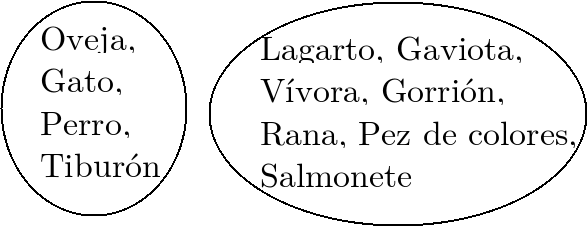
\includegraphics[width=0.5\textwidth]{figures/ejemplo1.png}}\\
  \subfloat[\emph{Ambiente donde viven}]{\label{fig:ejemplo2}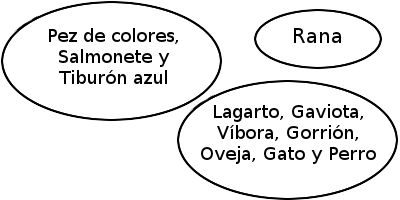
\includegraphics[width=0.5\textwidth]{figures/ejemplo2.png}}
  \caption{Clustering de acuerdo a diferentes criterios}
  \label{fig:ejemplos}
\end{figure}

%Se puede ver que gracias a la falta de un criterio universal para el clustering,
% \'esta es muy subjetiva en muchos casos.
\item Es importante entender la diferencia
entre clustering (aprendizaje no supervisado) y clasificación supervisada. 
En esta última, se tiene una colección de patrones etiquetados
(pre-clasificados) y se quiere etiquetar un nuevo patrón encontrado.
Típicamente, los patrones ya etiquetados son usados para obtener
las descripciones de las clases, que a su vez se utilizan para etiquetar el
nuevo patrón.
%Se puede ver desde el punto de vista de aprendizaje autom\'atico, donde los clusters
%correponden a patrones escondidos en los datos, la b\'usqueda de clusters 
%es una especie de aprendizaje no supervisado. 
En el caso de clustering, el problema consiste en agrupar una colección de
patrones no etiquetados en grupos significativos. En este sentido, las etiquetas
se asocian con los clusters.

\item Se espera que un algoritmo de clustering descubra el agrupamiento natural
que existe en conjunto de patrones o datos. Cada patrón puede ser identificado
como un punto en un hiper-espacio, llamado espacio de características. La entrada
del algoritmo es un conjunto de puntos del hiper-espacio característico. Un
algoritmo ideal de clustering debe tener como salida, la etiqueta de cada
patrón, es decir, el grupo al cual pertenece.
\end{itemize}

\pagebreak
	Este problema ha sido abordado por diversos campos del conocimiento como la
estadística (análisis multivariado), teoría de grafos, computación evolutiva,
redes neuronales, entre otros\cite{SwAjAm2009}. Algunas de sus aplicaciones son
la minería de datos, segmentaciones de clientes, recuperación de documentos y
procesamiento de imágenes \cite{GaChJi2007}. En especial, llama la atención el
último campo mencionado. El procesamiento de imágenes es muy útil para los
humanos. Su importancia radica en que, el resultado de hacer clustering a una
imagen, puede ser usado como la entrada para un modelo basado en sistemas de
reconocimiento de objetos. También, en el área médica, puede ayudar a encontrar
regiones en las imágenes que sean de interés.

%Actualmente existe una amplia investigaci\'on sobre la aplicaci\'on de distintas metaheur\'isticas para
%resolver diversos problemas optimizaci\'on. La idea es encontrar en un tiempo
%razonable la respuesta \'optima o una lo m\'as cercana a ella. Muchos cient\'ificos han empezado a inspirarse en la naturaleza.
%Una profunda obsevaci\'on en la relaci\'on subyacente 
%entre la naturaleza y optimizaci\'on ha llevado al desarrollo de nuevos paradigmas
%para lograr este objetivo\cite{SwAjAm2009}. De ac\'a surgen las basadas en poblaci\'on e inteligencia
%colectiva.
Actualmente existe una amplia investigación sobre la aplicación de distintas
metaheurísticas para resolver diversos problemas optimización. La idea es
encontrar en un tiempo razonable la respuesta óptima o cercana a ella. Muchos
científicos, inspirándose en la naturaleza, han encontrado una relación
subyacente entre ésta y la optimización lo cual ha propiciado el desarrollo de
nuevos paradigmas para lograr este objetivo\cite{SwAjAm2009}. Así que surgen las
metaheurísticas basadas en población e inteligencia colectiva.

%Las m\'as conocidas y prometedoras son el algoritmo g\'enetico, la abeja, la evoluci\'on diferencial(DE), la hormiga
%y el optimizador de enjambre de part\'iculas (PSO). Todos constan de un grupo de individuos que van a ir modificandose a trav\'es
%del tiempo. La forma en que se den estos cambios depende de cada algoritmo.
Las metaheurísticas más conocidas y prometedoras son el algoritmo genético, de
abeja y hormiga, el optimizador de enjambre de partículas, la evolución
diferencial. Todas estas metaheurísticas funcionan con un grupo de individuos
(soluciones) que se modifican a lo largo de la ejecución de las mismas. La forma
en que se den estos cambios depende de cada algoritmo.

Para este trabajo, se implementaron siete metaheurísticas y el algoritmo
determinista \emph{K-means} para resolver el problema de \emph{data clustering}
y se realizó un estudio comparativo de sus desempeños.
La entonación de los parámetros de cada metaheurística se realizó utilizando un
esquema de trabajo basado en el diseño de experimentos; adicionalmente, se
intentó utilizar el análisis de varianza para determinar los parámetros que
tienen mayor influencia en el desempeño de cada metaheurísticas y así orientar
el proceso de entonación. El objetivo principal que se busca es identificar las
metaheurísticas que mejor resuelven el problema de clustering de datos numéricos.

Este documento se encuentra organizado de la siguiente manera: en el primer
capítulo, se tratan los algoritmos de optimización tradicionales y no
tradicionales, además se describen de manera general las metaheurística
implementadas. En el segundo capítulo, se define el problema de cluster y los
índices de validez usados para la comparación de las metaheurísticas. En el 
tercer capítulo, se describen los detalles de implementación de cada
metaheurística implementada. En el cuarto capítulo, se realiza un análisis
comparativo de los resultados obtenidos. Finalmente, en el quito capítulo, se
presentan las conclusiones y las recomendaciones para trabajos de investigación
futuros.
\end{comment}
